\documentclass[10pt]{article}

\usepackage[utf8]{inputenc}
\usepackage[spanish]{babel}
\decimalpoint
\usepackage{amsmath, amssymb}
\usepackage{xcolor}
\usepackage{geometry}
\geometry{letterpaper, margin=1in}
\usepackage{graphicx}
\usepackage{float}
\usepackage{array}
\usepackage{booktabs}
\usepackage{colortbl}
\usepackage{caption}
\usepackage{tocloft}

\usepackage[colorlinks=true, linkcolor=black, urlcolor=black, citecolor=black]{hyperref}
%%%%%%%%%%%%%%%%%%%%%%%%%%%%%%%%%%%%%%%%%%%%%%%%%%%%%%%%%%%%%%%%%%%%%%%%%%%%%%%%%%%%%%%%%%%%%%%%%%%%%%%%%%%%%%
%%%%%%%%%%%%%%%%%%%%%%%%%%%%%%%%%%%%%%%%%%%%%%%%%%%%%%%%%%%%%%%%%%%%%%%%%%%%%%%%%%%%%%%%%%%%%%%%%%%%%%%%%%%%%%
\title{Universidad Panamericana \\ Maestría en Ciencia de Datos \\ Datos Masivos \\ 
    \vspace{0.5cm} Proyecto Final: \textit{Monitoreo Inteligente de Tráfico Marítimo con Big Data AIS}}
\author{Enrique Ulises Báez Gómez Tagle, Luis Alejandro Guillén Alvarez}
\date{\today}
%%%%%%%%%%%%%%%%%%%%%%%%%%%%%%%%%%%%%%%%%%%%%%%%%%%%%%%%%%%%%%%%%%%%%%%%%%%%%%%%%%%%%%%%%%%%%%%%%%%%%%%%%%%%%%
%%%%%%%%%%%%%%%%%%%%%%%%%%%%%%%%%%%%%%%%%%%%%%%%%%%%%%%%%%%%%%%%%%%%%%%%%%%%%%%%%%%%%%%%%%%%%%%%%%%%%%%%%%%%%%
%%%%%%%%%%%%%%%%%%%%%%%%%%%%%%%%%%%%%%%%%%%%%%%%%%%%%%%%%%%%%%%%%%%%%%%%%%%%%%%%%%%%%%%%%%%%%%%%%%%%%%%%%%%%%%%%%%%%%%%%%%%%%%%%%%%%%%%%%%%%%%%%%%%%%%%%%%%%%%%%%%%%%%%%%%%%%%%%%%%%%%%%%%%%%%
%%%%%%%%%%%%%%%%%%%%%%%%%%%%%%%%%%%%%%%%%%%%%%%%%%%%%%%%%%%%%%%%%%%%%%%%%%%%%%%%%%%%%%%%%%%%%%%%%%%%%%%%%%%%%%%%%%%%%%%%%%%%%%%%%%%%%%%%%%%%%%%%%%%%%%%%%%%%%%%%%%%%%%%%%%%%%%%%%%%%%%%%%%%%%%
\begin{document}

\maketitle

\tableofcontents

\newpage

%%%%%%%%%%%%%%%%%%%%%%%%%%%%%%%%%%%%%%%%%%%%%%%%%%%%%%%%%%%%%%%%%%%%%%%%%%%%%%%%%%%%%%%%%%%%%%%%%%%%%%%%%%%%%%%%%%%%%%%%%%%%%%%%%%%%%%%%%%%%%%%%%%%%%%%%%%%%%%%%%%%%%%%%%%%%%%%%%%%%%%%%%%%%%%
%%%%%%%%%%%%%%%%%%%%%%%%%%%%%%%%%%%%%%%%%%%%%%%%%%%%%%%%%%%%%%%%%%%%%%%%%%%%%%%%%%%%%%%%%%%%%%%%%%%%%%%%%%%%%%%%%%%%%%%%%%%%%%%%%%%%%%%%%%%%%%%%%%%%%%%%%%%%%%%%%%%%%%%%%%%%%%%%%%%%%%%%%%%%%%
\section{Resumen ejecutivo}
\subsection{Introducción} % REVISIÓN GUILLÉN 

El tráfico marítimo global genera millones de registros de posicionamiento a través del Sistema de Identificación Automática (AIS), que transmite automáticamente la identidad, posición, velocidad y otros datos de los buques. Originalmente implementado para mejorar la seguridad de la navegación, hoy es crucial para la gestión del tráfico marítimo, la conciencia del entorno y operaciones de búsqueda y rescate.

Este proyecto propone aprovechar Big Data y aprendizaje automático (ML) para analizar una base de datos masiva de mensajes AIS y ofrecer una solución innovadora a la pregunta: \textbf{¿Cómo detectar y entender comportamientos anómalos en el tráfico marítimo para mejorar la seguridad y la eficiencia?}

Responder esta pregunta implica analizar patrones normales de navegación y descubrir desviaciones significativas. En esencia:
\begin{itemize}
    \item \textbf{¿Qué estamos haciendo?} Diseñamos un sistema de análisis que procesa grandes volúmenes de datos AIS para identificar anomalías en el comportamiento de los buques (posiciones fuera de lugar, velocidades inusuales, maniobras erráticas, etc.) y extraer patrones útiles sobre la operación de diferentes tipos de embarcaciones.
    \item \textbf{¿Para qué lo hacemos?} Para mejorar la seguridad marítima, la gestión del tráfico y la toma de decisiones, ofreciendo alertas tempranas de potenciales riesgos (colisiones, actividades ilícitas o fallos) y conocimiento profundo a autoridades y empresas navieras.
    \item \textbf{¿Cómo lo hacemos?} Empleando herramientas de Big Data de la Suite de Google Cloud (Storage + DataProc + BigQuery) para procesar datos geoespaciales masivos en en poco tiempo, complementado con modelos de ML que aprenden patrones habituales y detectan comportamientos que se apartan de lo normal.
    \item \textbf{¿A quién beneficia?} A organismos de seguridad marítima (marinas, guardacostas), a empresas navieras optimizando rutas y monitoreo de flotas, a aseguradoras evaluando riesgos operativos e incluso a investigadores del medio marino en estudios ecológicos.
\end{itemize}

Finalmente, los resultados se integraron en un \textit{dashboard} interactivo con visualizaciones (mapas geográficos, gráficos de tendencias y rankings) que facilitan la interpretación y la toma de decisiones.
%%%%%%%%%%%%%%%%%%%%%%%%%%%%%%%%%%%%%%%%%%%%%%%%%%%%%%%%%%%%%%%%%%%%%%%%%%%%%%%%%%%%%%%%%%%%%%%%%%%%%%%%%%%%%%%%%%%%%%%%%%%%%%%%%%%%%%%%%%%%%%%%%%%%%%%%%%%%%%%%%%%%%%%%%%%%%%%%%%%%%%%%%%%%%%
%%%%%%%%%%%%%%%%%%%%%%%%%%%%%%%%%%%%%%%%%%%%%%%%%%%%%%%%%%%%%%%%%%%%%%%%%%%%%%%%%%%%%%%%%%%%%%%%%%%%%%%%%%%%%%%%%%%%%%%%%%%%%%%%%%%%%%%%%%%%%%%%%%%%%%%%%%%%%%%%%%%%%%%%%%%%%%%%%%%%%%%%%%%%%%
\section{Visión general del desarrollo} 
\subsection{Solución Actual / visión general} % REVISIÓN GUILLÉN: FALTA AÑADIR PARTE DE ML tanto descripción como diagrama

La solución actual se implementa de extremo a extremo sobre la nube de Google Cloud. El flujo completo es el siguiente:

\begin{itemize}
    \item Una máquina virtual en Google Compute Engine se encarga de \textbf{scrapear los datos AIS} y cargarlos en Google Cloud Storage. 
    \item En Cloud Storage se organizan dos capas diferenciadas: \textit{raw} y \textit{curated}, con prefijos de carpeta y particiones por mes (\texttt{YYYY-MM=}).
    \item Un clúster de Google Cloud DataProc ejecuta dos jobs:
    \begin{itemize}
        \item Job \textbf{raw}: descomprime los archivos obtenidos y organiza los datos en particiones por año y mes, y finalmente los guarda en formato Parquet en Google Cloud Storage.
        \item Job \textbf{curated}: lee la capa cruda, aplica transformaciones iniciales y genera la capa refinada lista para análisis.
    \end{itemize}
    \item Una Cloud Function crea el \textbf{dataset y la tabla en BigQuery}, cargando la información desde la capa curated.
    \item En BigQuery se centraliza la explotación de datos mediante consultas SQL optimizadas, generando los datasets finales que alimentan las visualizaciones.
    \item El \textbf{dashboard de Streamlit}, desplegado en la misma VM, consume los resultados de BigQuery y presenta mapas, gráficos de tendencias y rankings de manera interactiva.
\end{itemize}

Toda la solución se ejecuta en la región \texttt{us-central1}. Para evitar duplicados en el flujo, se utiliza la clave compuesta \textbf{MMSI + timestamp}.
\vspace{0.5cm}
\begin{figure}[H]
    \centering
    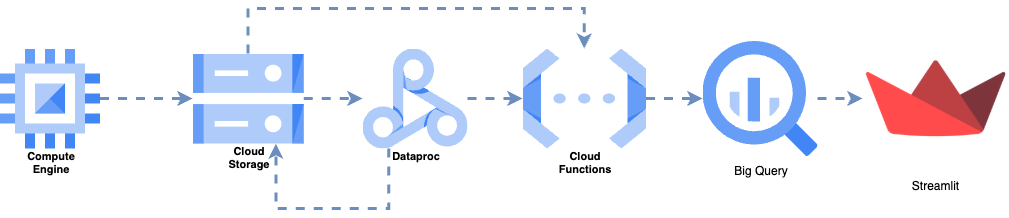
\includegraphics[width=\textwidth]{figures/arch/ArchitectureDiagram.png}
    \caption{Arquitectura actual de la solución: flujo end-to-end en Google Cloud.}
\end{figure}
\vspace{0.1cm}
%%%%%%%%%%%%%%%%%%%%%%%%%%%%%%%%%%%%%%%%%%%%%%%%%%%%%%%%%%%%%%%%%%%%%%%%%%%%%%%%%%%%%%%%%%%%%%%%%%%%%%%%%%%%%%%%%%%%%%%%%%%%%%%%%%%%%%%%%%%%%%%%%%%%%%%%%%%%%%%%%%%%%%%%%%%%%%%%%%%%%%%%%%%%%%
%%%%%%%%%%%%%%%%%%%%%%%%%%%%%%%%%%%%%%%%%%%%%%%%%%%%%%%%%%%%%%%%%%%%%%%%%%%%%%%%%%%%%%%%%%%%%%%%%%%%%%%%%%%%%%%%%%%%%%%%%%%%%%%%%%%%%%%%%%%%%%%%%%%%%%%%%%%%%%%%%%%%%%%%%%%%%%%%%%%%%%%%%%%%%%
\subsection{Limitaciones actuales de la solución} % REVISAR: KIKE

Actualmente la solución no está implementada de manera completamente \textit{event-driven}. 
El disparo de los diferentes procesos (por ejemplo, la ejecución de la Cloud Function tras la escritura en la capa \textbf{curated}) no se encuentra automatizado mediante eventos de GCS o Pub/Sub, 
sino que requiere pasos manuales o ejecución programada. 
Esto representa una limitación en términos de eficiencia y escalabilidad. 
Como mejora futura se plantea migrar a un esquema \textbf{event-driven}, en el cual cada etapa del pipeline se active automáticamente al completarse la anterior, reduciendo la intervención manual y acelerando el flujo de datos de extremo a extremo.

%%%%%%%%%%%%%%%%%%%%%%%%%%%%%%%%%%%%%%%%%%%%%%%%%%%%%%%%%%%%%%%%%%%%%%%%%%%%%%%%%%%%%%%%%%%%%%%%%%%%%%%%%%%%%%%%%%%%%%%%%%%%%%%%%%%%%%%%%%%%%%%%%%%%%%%%%%%%%%%%%%%%%%%%%%%%%%%%%%%%%%%%%%%%%%
%%%%%%%%%%%%%%%%%%%%%%%%%%%%%%%%%%%%%%%%%%%%%%%%%%%%%%%%%%%%%%%%%%%%%%%%%%%%%%%%%%%%%%%%%%%%%%%%%%%%%%%%%%%%%%%%%%%%%%%%%%%%%%%%%%%%%%%%%%%%%%%%%%%%%%%%%%%%%%%%%%%%%%%%%%%%%%%%%%%%%%%%%%%%%%
\subsection{Propósito, uso y alcance de la herramienta} % TODO: GUILLÉN
%%%%%%%%%%%%%%%%%%%%%%%%%%%%%%%%%%%%%%%%%%%%%%%%%%%%%%%%%%%%%%%%%%%%%%%%%%%%%%%%%%%%%%%%%%%%%%%%%%%%%%%%%%%%%%%%%%%%%%%%%%%%%%%%%%%%%%%%%%%%%%%%%%%%%%%%%%%%%%%%%%%%%%%%%%%%%%%%%%%%%%%%%%%%%%
\section{Revisión y uso de datos}
\subsection{Orígenes y control de datos} % REVISIÓN GUILLÉN

Los datos utilizados provienen del portal oficial de la NOAA (\url{https://coast.noaa.gov/htdata/CMSP/AISDataHandler/2024/index.html}), el cual publica archivos comprimidos (.zip) con los mensajes AIS recolectados a lo largo del año 2024. 
Para garantizar la trazabilidad y el control de los datos, se desarrolló un script en Python (\texttt{scrapper.py}) que automatiza la descarga de todos los archivos disponibles, verificando duplicados mediante el tamaño de los ficheros y evitando descargas innecesarias. 
De esta manera se asegura que la totalidad de los datos originales publicados por la NOAA sean capturados sin alteración.

%%%%%%%%%%%%%%%%%%%%%%%%%%%%%%%%%%%%%%%%%%%%%%%%%%%%%%%%%%%%%%%%%%%%%%%%%%%%%%%%%%%%%%%%%%%%%%%%%%%%%%%%%%%%%%%%%%%%%%%%%%%%%%%%%%%%%%%%%%%%%%%%%%%%%%%%%%%%%%%%%%%%%%%%%%%%%%%%%%%%%%%%%%%%%%
\subsection{Preparación de datos} % REVISIÓN GUILLÉN

La preparación de los datos comienza en una máquina virtual de Google Compute Engine, donde se ejecuta el script de scraping. Este proceso descarga en paralelo (con \textit{threads}) todos los archivos .zip hacia un directorio local (\texttt{ais\_2024}) y posteriormente los transfiere a Google Cloud Storage en la capa \textbf{raw}. 

\paragraph{Resumen de etapas (alto nivel).}
El pipeline de preparación contempla dos jobs en DataProc que operan sobre Cloud Storage:
\begin{enumerate}
  \item \textbf{RAW\_INGEST} (ingesta a \textit{raw}): descomprime lotes \texttt{.zip} provenientes del scraping y los convierte a formato Parquet \emph{particionado por mes} (columna derivada \texttt{ym}), añadiendo trazabilidad mínima (archivo fuente y timestamp de ingesta).
  \item \textbf{CURATED\_TRANSFORMATIONS} (hacia \textit{curated}): toma la salida \textit{raw} y aplica transformaciones básicas para dejar un esquema uniforme y listo para consumo analítico (normalizaciones de tipos, columnas temporales y desduplicación por \texttt{MMSI+BaseDateTime}).
\end{enumerate}
Para mayor detalle, los detalles finos de limpieza, reglas y enriquecimientos revisar en la sección \textit{Limpieza y tratamiento de datos}.

\paragraph{Automatización hacia BigQuery (Cloud Function).}
Tras la generación de la capa \textbf{curated} en Cloud Storage, una Cloud Function automatiza la creación/verificación de \textbf{datasets} y \textbf{tablas} en BigQuery. Su lógica principal es idempotente:
\begin{itemize}
    \item Si la tabla ya existe, responde \texttt{action: none}.
    \item Si no existe y no se proporcionó esquema, intenta \textbf{autodetectarlo} cargando una muestra desde \texttt{gcs\_uri}. Soporta formatos \textit{Parquet/CSV/JSON/Avro/ORC} y versiones comprimidas (\texttt{.gz/.bz2/.zst}).
    \item Si se proporciona \texttt{schema}, crea la tabla con ese esquema explícito.
\end{itemize}
En la solución actual, esta función se integra al final del ETL, tras DataProc, para que la capa \textbf{curated} quede disponible en BigQuery lista para explotación y consumo por el dashboard.
%%%%%%%%%%%%%%%%%%%%%%%%%%%%%%%%%%%%%%%%%%%%%%%%%%%%%%%%%%%%%%%%%%%%%%%%%%%%%%%%%%%%%%%%%%%%%%%%%%%%%%%%%%%%%%%%%%%%%%%%%%%%%%%%%%%%%%%%%%%%%%%%%%%%%%%%%%%%%%%%%%%%%%%%%%%%%%%%%%%%%%%%%%%%%%
\subsection{Limpieza y tratamiento de datos} % REVISIÓN GUILLÉN 

En esta sección se describen de manera detallada las transformaciones y criterios aplicados para convertir los datos AIS en una capa \textbf{curated} funcional para el análisis. Se listan los pasos con su \emph{porqué} operativo o estadístico.

\paragraph{Normalizaciones y tipos.}
\begin{itemize}
  \item \textbf{Casteo y estandarización}: se convierten columnas numéricas a tipos adecuados (\texttt{double}/\texttt{int}) y se normalizan textos (\texttt{trim}, mayúsculas controladas) para evitar variabilidad en joins/agrupaciones.
  \item \textbf{Timestamps en UTC}: \texttt{BaseDateTime} se parsea a tipo timestamp con zona UTC para análisis temporales coherentes; sobre esta base se derivan \texttt{date}, \texttt{hour}, \texttt{week}, \texttt{month}, \texttt{quarter} y una columna \texttt{ym} (AAAA-MM) para particionado.
\end{itemize}

\paragraph{Coordenadas y límites físicos.}
\begin{itemize}
  \item \textbf{LAT/LON válidos}: se recortan latitudes al rango [-90, 90] y longitudes se \emph{envuelven} a [-180, 180] (corrigiendo valores fuera de dominio por errores/reporte). Se descartan registros con coordenadas nulas tras la corrección.
  \item \textbf{Redondeo razonable}: se redondean LAT/LON a 5 decimales para homogenizar precisión sin perder resolución náutica relevante.
\end{itemize}

\paragraph{Velocidad, rumbos y estados.}
\begin{itemize}
  \item \textbf{SOG (Speed Over Ground)}: se acota a [0, 70] nudos para eliminar outliers físicos/telemetría corrupta; adicionalmente se calcula \texttt{SOG\_ms} en m/s para modelos.
  \item \textbf{COG/Heading}: se normaliza módulo 360°. El valor \texttt{Heading=511} (no disponible) se marca como nulo para evitar sesgos en métricas de rumbo.
  \item \textbf{NavStatus}: se genera \texttt{NavStatusInt} a partir de \texttt{Status} y se une contra un catálogo para \texttt{NavStatusName}; códigos fuera de 0–15 se etiquetan como \textit{Unknown} y faltantes como \textit{Not reported}.
\end{itemize}

\paragraph{Dimensiones y calado.}
\begin{itemize}
  \item \textbf{Length/Width}: se acotan a rangos plausibles (1–450 m y 1–70 m, respectivamente) para descartar errores de orden de magnitud.
  \item \textbf{Draft}: se limita a [0, 25] m; valores negativos o excesivos suelen provenir de carga mal reportada o errores de parsing.
\end{itemize}

\paragraph{Identificadores y texto.}
\begin{itemize}
  \item \textbf{MMSI}: se extrae la porción numérica válida (1–9 dígitos) y se rellena a 9 con ceros a la izquierda para formato consistente.
  \item \textbf{IMO/CallSign/VesselName}: se normalizan espacios y caracteres no alfanuméricos; se limpian IMOs genéricos (p.ej., \texttt{IMO0000000}, \texttt{0}, vacío) para evitar falsas uniones.
\end{itemize}

\paragraph{Clasificación de tipo de buque.}
\begin{itemize}
  \item \textbf{VesselType}: se derivan \texttt{VesselTypeInt}, \texttt{VesselTypeName} (mediante mapa IMO) y \texttt{VesselTypeClass} (WIG, Cargo, Tanker, Passenger, etc.). Esto permite comparar métricas por clase homogénea y soportar reglas dependientes del tipo.
\end{itemize}

\paragraph{Enriquecimiento geoespacial.}
\begin{itemize}
  \item \textbf{Geohash9}: se calcula un \texttt{geohash9} distribuido (UDF con \texttt{pygeohash}) para agregación espacial eficiente y enlaces a capas geográficas (vallas, puertos, TSS) en análisis posteriores.
\end{itemize}

\paragraph{Calidad e idempotencia.}
\begin{itemize}
  \item \textbf{Desduplicación}: se eliminan duplicados por clave compuesta \texttt{(MMSI, BaseDateTime)} para asegurar series temporales limpias por embarcación.
  \item \textbf{Validación de conteos}: en \textit{raw}, se comparan conteos diarios (CSV vs Parquet) y se aborta si no coinciden; en \textit{curated}, se escriben marcadores de éxito por partición (\texttt{\_markers/ym=.../\_SUCCESS}) para reanudación y ejecución incremental sin sobrescribir trabajo correcto.
\end{itemize}
%%%%%%%%%%%%%%%%%%%%%%%%%%%%%%%%%%%%%%%%%%%%%%%%%%%%%%%%%%%%%%%%%%%%%%%%%%%%%%%%%%%%%%%%%%%%%%%%%%%%%%%%%%%%%%%%%%%%%%%%%%%%%%%%%%%%%%%%%%%%%%%%%%%%%%%%%%%%%%%%%%%%%%%%%%%%%%%%%%%%%%%%%%%%%%
\subsection{Integridad de los datos} % TODO: GUILLÉN
%%%%%%%%%%%%%%%%%%%%%%%%%%%%%%%%%%%%%%%%%%%%%%%%%%%%%%%%%%%%%%%%%%%%%%%%%%%%%%%%%%%%%%%%%%%%%%%%%%%%%%%%%%%%%%%%%%%%%%%%%%%%%%%%%%%%%%%%%%%%%%%%%%%%%%%%%%%%%%%%%%%%%%%%%%%%%%%%%%%%%%%%%%%%%%
\subsection{Limitaciones de los datos} % TODO: GUILLÉN
%%%%%%%%%%%%%%%%%%%%%%%%%%%%%%%%%%%%%%%%%%%%%%%%%%%%%%%%%%%%%%%%%%%%%%%%%%%%%%%%%%%%%%%%%%%%%%%%%%%%%%%%%%%%%%%%%%%%%%%%%%%%%%%%%%%%%%%%%%%%%%%%%%%%%%%%%%%%%%%%%%%%%%%%%%%%%%%%%%%%%%%%%%%%%%
\section{Proceso de desarrollo}
\subsection{Metodología} % REVISIÓN GUILLÉN 

La metodología seguida para el proyecto se basa en un pipeline de datos con varias etapas bien definidas. En la primera etapa, una VM en Google Compute Engine ejecuta el módulo de scraping, encargado de descargar automáticamente los archivos AIS de la NOAA y trasladarlos a la nube (Cloud Storage). 
A partir de ahí, se desencadenan las siguientes fases: procesamiento con DataProc, almacenamiento en diferentes capas (raw y curated), carga a BigQuery y visualización con Streamlit. 
De esta manera, la metodología integra la automatización de la recolección de datos como un paso fundamental previo al procesamiento distribuido.

\paragraph{Proceso de desarrollo.}
\begin{itemize}
  \item \textbf{Orquestación y repetibilidad}: los jobs se ejecutan en DataProc con configuraciones de tolerancia a fallos (speculation, retries) y \emph{idempotencia} (partition overwrite dinámico + marcadores). Esto permite relanzar sin duplicar datos ni romper particiones.
  \item \textbf{Particionado y costos}: todas las salidas en GCS se particionan por \texttt{ym} (AAAA-MM), lo que luego se refleja en BigQuery para escaneos selectivos y costos predecibles.
  \item \textbf{Versionamiento de dependencias}: se distribuyen "wheels" (p.ej., \texttt{pygeohash}) y un entorno reproducible (tarball de venv) a los ejecutores vía \texttt{spark.yarn.dist.archives}, garantizando que las UDFs geoespaciales funcionen de forma consistente.
  \item \textbf{Observabilidad}: se registran conteos globales y por día, así como tiempos de etapa, para detectar desviaciones (picos inusuales, lag IO). Los logs documentan causas de fallas y se retienen para auditoría.
  \item \textbf{Publicación a BigQuery}: una vez escrita la capa \textit{curated}, la Cloud Function verifica/crea dataset y tabla en \texttt{us-central1} y, de ser necesario, autodetecta esquema a partir de una muestra en GCS, dejando la data lista para explotación por el dashboard Streamlit.
\end{itemize}

\noindent\textit{Diferencia conceptual:} \textbf{Preparación de datos} resume \emph{qué} pasos iniciales se ejecutan (ingesta y preprocesos), mientras que \textbf{Proceso de desarrollo / Metodología} documenta \emph{cómo} se construye, ejecuta y asegura la calidad del pipeline (idempotencia, tolerancia a fallos, particionado, dependencias y publicación).

%%%%%%%%%%%%%%%%%%%%%%%%%%%%%%%%%%%%%%%%%%%%%%%%%%%%%%%%%%%%%%%%%%%%%%%%%%%%%%%%%%%%%%%%%%%%%%%%%%%%%%%%%%%%%%%%%%%%%%%%%%%%%%%%%%%%%%%%%%%%%%%%%%%%%%%%%%%%%%%%%%%%%%%%%%%%%%%%%%%%%%%%%%%%%%
\subsection{Pruebas} % TODO: GUILLÉN
%%%%%%%%%%%%%%%%%%%%%%%%%%%%%%%%%%%%%%%%%%%%%%%%%%%%%%%%%%%%%%%%%%%%%%%%%%%%%%%%%%%%%%%%%%%%%%%%%%%%%%%%%%%%%%%%%%%%%%%%%%%%%%%%%%%%%%%%%%%%%%%%%%%%%%%%%%%%%%%%%%%%%%%%%%%%%%%%%%%%%%%%%%%%%%
\section{Resultados y conclusiones} % TODO: GUILLÉN
%%%%%%%%%%%%%%%%%%%%%%%%%%%%%%%%%%%%%%%%%%%%%%%%%%%%%%%%%%%%%%%%%%%%%%%%%%%%%%%%%%%%%%%%%%%%%%%%%%%%%%%%%%%%%%%%%%%%%%%%%%%%%%%%%%%%%%%%%%%%%%%%%%%%%%%%%%%%%%%%%%%%%%%%%%%%%%%%%%%%%%%%%%%%%%
%%%%%%%%%%%%%%%%%%%%%%%%%%%%%%%%%%%%%%%%%%%%%%%%%%%%%%%%%%%%%%%%%%%%%%%%%%%%%%%%%%%%%%%%%%%%%%%%%%%%%%%%%%%%%%%%%%%%%%%%%%%%%%%%%%%%%%%%%%%%%%%%%%%%%%%%%%%%%%%%%%%%%%%%%%%%%%%%%%%%%%%%%%%%%%
\section{Código utilizado} % REVISIÓN GUILLÉN 
\subsection{Link al repositorio con código fuente y salidas correspondientes}
\url{https://github.com/enriquegomeztagle/MCD-BigData-SmartMaritimeTrafficMonitoring-FinalProject}
%%%%%%%%%%%%%%%%%%%%%%%%%%%%%%%%%%%%%%%%%%%%%%%%%%%%%%%%%%%%%%%%%%%%%%%%%%%%%%%%%%%%%%%%%%%%%%%%%%%%%%%%%%%%%%%%%%%%%%%%%%%%%%%%%%%%%%%%%%%%%%%%%%%%%%%%%%%%%%%%%%%%%%%%%%%%%%%%%%%%%%%%%%%%%%
%%%%%%%%%%%%%%%%%%%%%%%%%%%%%%%%%%%%%%%%%%%%%%%%%%%%%%%%%%%%%%%%%%%%%%%%%%%%%%%%%%%%%%%%%%%%%%%%%%%%%%%%%%%%%%%%%%%%%%%%%%%%%%%%%%%%%%%%%%%%%%%%%%%%%%%%%%%%%%%%%%%%%%%%%%%%%%%%%%%%%%%%%%%%%%
\end{document}
%%%%%%%%%%%%%%%%%%%%%%%%%%%%%%%%%%%%%%%%%%%%%%%%%%%%%%%%%%%%%%%%%%%%%%%%%%%%%%%%%%%%%%%%%%%%%%%%%%%%%%%%%%%%%%%%%%%%%%%%%%%%%%%%%%%%%%%%%%%%%%%%%%%%%%%%%%%%%%%%%%%%%%%%%%%%%%%%%%%%%%%%%%%%%%
